\documentclass[a4paper,12pt]{article}
\usepackage[margin=1in]{geometry}
\renewcommand{\tabcolsep}{1 mm}
\usepackage[T2A]{fontenc}			% кодировка
\usepackage[utf8]{inputenc}			% кодировка исходного текста
\usepackage[english,russian]{babel}	% локализация и переносы
\usepackage{graphicx}                % Математика
\usepackage{amsmath,amsfonts,amssymb,amsthm,mathtools} 
\usepackage{mathtext}
\usepackage[T2A]{fontenc}
\usepackage[utf8]{inputenc}

\usepackage{wasysym}

%Заговолок
\author{Бичина Марина 
группа Б04-005 1 курса ФЭФМ}
\title{Отчет по лабораторной работе №2.5.1


Измерение коэффициента поверхностного натяжения жидкости}
\date{15.04.2021}


\begin{document} % начало документа
\renewcommand{\labelenumii}{\arabic{enumii})}
\maketitle
\newpage

\section{Аннотация}

\paragraph{Цель работы:} 
\begin{enumerate}
\itemsep0em
\item Измерить температурную зависимость  коэффициента поверхностного натяжения дистиллированной воды с использованием известного коэффициента поверхностного натяжения спирта;
\item Определить полную поверхностную энергию  и теплоту, необходимые для изотермического образования единицы  поверхности жидкости  при различной температуре
\end{enumerate}
\paragraph{Оборудование:}
\begin{enumerate}
\itemsep0em
\item прибор Ребиндера с термостатом и микроманометром
\item исследуемые жидкости
\item стаканы
\end{enumerate}
\section{Теоретическая часть}

\paragraph{} Наличие поверхностного слоя приводит к различию давлений по разные стороны от искривленной границы раздела двух сред.  Для сферического пузырька с воздухом  внутри жидкости избыточное давление даётся формулой Лапласа:
\begin{equation}
\Delta P = P _{\text{внутри}} - P_{ \text{снаружи}} = \dfrac{2 \sigma}{r}
\label{laplass}
\end{equation}
где 
\begin{enumerate}
\itemsep0em
\item $\sigma$ -- коэффициент поверхностного натяжения
\item $P _{\text{внутри}}, P_{ \text{снаружи}}$  -- давление внутри пузырька и снаружи
\item $r$ -- радиус кривизны поверхности раздела двух фаз
\end{enumerate}
Эта формула лежит в основе предлагаемого метода определения коэффициента поверхностного натяжения жидкости. Измеряется давление $\Delta P$, необходимое для выталкивания в жидкость пузырька воздуха.
\subsection{Описание установки:}

\begin{figure}[h]
\begin{center}
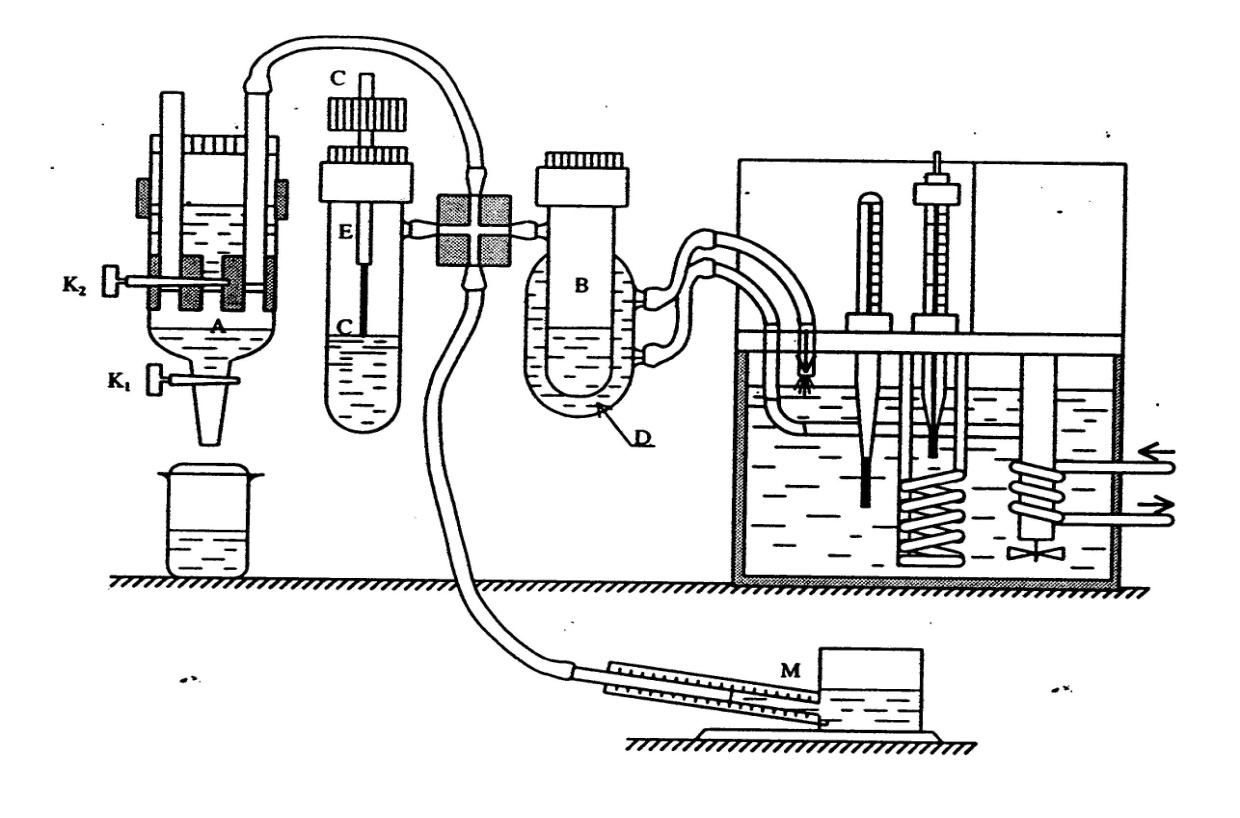
\includegraphics[width=0.5\linewidth]{ustanovka_1.png}
\caption{Схема установки для измерения температурной зависимости
коэффициента поверхностного натяжения}
\label{ris:ustanovka_1} 
\end{center}
\end{figure}
Исследуемая жидкость (дистиллированная вода) наливается в сосуд (колбу) В (см рисунок \ref{ris:ustanovka_1}). Тестовая жидкость  (этиловый спирт) наливается  в сосуд Е.  При измерениях  колбы герметично закрываются  пробками.   Через одну из двух пробок  проходит полая металлическая игла С. Этой пробкой закрывается сосуд, в котором  проводятся измерения. Верхний конец иглы открыт в атмосферу, а нижний погружен в жидкость. Другой сосуд герметично закрывается второй пробкой. При создании достаточного  разряжения воздуха в колбе с иглой пузырьки воздуха начинают пробулькивать через жидкость. Поверхностное натяжение можно определить по величине разряжения $\Delta P$ (по формуле \ref{laplass}), необходимого для прохождения пузырьков (при известном радиусе иглы).

Разряжение в системе создается с помощью аспиратора А. Кран $K_2$ разделяет две полости аспиратора. Верхняя полость при закрытом кране $K_2$  заполняется водой. Затем кран $K_2$ открывают и заполняют водой  нижнюю полость  аспиратора.  Разряжение воздуха создается в нижней полости  при открывании крана $K_1$, когда  вода вытекает из неё по каплям. В колбах В и С, соединённых трубками с нижней полостью аспиратора,  создается такое же пониженное давление. Разность давлений в полостях с разряженным воздухом и атмосферой измеряется спиртовым микроманометром Полное давление, измеренное при этом микроманометром,равно $P = \Delta P + \rho gh$

\subsection{Контрольные вопросы:}
\begin{enumerate}
\itemsep0em
\item\textbf{ Если пропускать несколько пузырьков в секунду, манометр показывает практически постоянное давление. Почему бы не измерять его?}\\
Если пропускать несколько пузырьков в секунду, то на манометре будет показано разряжение, при котором в равновесие приходит количество вещества, приходящее с пузырьками, и скорость создания разряжения. Для того, чтобы пузырьки быстро образовывались друг за другом, необходимо, чтобы воздух, приносимых одним пузырьком не уменьшал разряжение до уровня, недостаточного для создания пузырька, значит в этот момент будет создано разряжение большее, чем необходимо для создание одного пузырька 
\item  \textbf{Почему следует измерять именно максимальное давление?}\\
При максимальном давлении идет образование пузырька, поскольку при меньших давлениях не преодолевается разность между гидростатическим давлением и лаплассовым. Далее энергия, которую пузырек несет в себе рассеивается, давление падает и мы не можем в таком случае точно установить коэффициент поверхностного натяжения.
\item \textbf{Почему погружение иглы уменьшает влияние теплового  расширения?}\\
Гидростатическое давление $\rho gh$ от температуры практически не зависит, поскольку подъем уровня жидкости компенсируется уменьшением ее плотности (из закона сохранения массы)
\item  \textbf{Почему пузырьки не должны касаться дна?} \\
В этом случае:\\
а) происходят деформации пузырька, которые усложнят расчеты (например, придется учитывать коэффициент смачивания стекла водой)\\
б) придется учитывать трение, которые может возникнуть между стенками сосуда и оболочкой пузырька \\
\item \textbf{Можно ли не зная глубины погружения иглы, определить $\sigma$, измеряя максимальное и минимальное давление при проталкивании пузырька?}
\item\textbf{ Пользуясь полученными результатами, оценить критическую температуру воды.} \\
Критическую температуру можно расчитать по формуле: 
\[T_{kr} = T_1 - \dfrac{\sigma}{\frac{d\sigma}{dT}} = 294 + \dfrac{62,01}{0,09} = 980 \;\; K\]
(На основании наших экспериментальных данных)
\item \textbf{Позволяет ли проведенный эксперимент заметить нелинейность зависимости $\sigma (T)$?\\}
Нет, в данном диапазоне температур данные хорошо аппроксимируются прямой $\sigma = a +bT$, поскольку температура довольна далека от критического значения 
\item \textbf{Какие погрешности преобладают в эксперименте: случайные или систематические?}\\
Случайные погрешности могут играть роль только в случае, если у нас всего 3 измерения. Если брать хотя бы 5 измерений, роль случайных погрешностей становится совсем невелика, поскольку мы не учитываем:\\
а) неидельность формы пузырька\\
б) тепловое расширение иглы\\
в) эффекты, связанные с теплопроводностью трубки, из-за которых температура на конце трубки заметно ниже, чем в глубине жидкости\\
г) неполное тепловое равновесие воды и термостата\\
А значения почти не отклонялись друг от друга, поэтому случайная погрешность невелика
\item \textbf{Какая величина должна стоять в формуле для высоты поднятия воды в стеклянном капилляре: $\sigma_{\text{вода - воздух}}$ или $\sigma_{\text{вода - стекло}}$?} \\
\[h = \dfrac{2\sigma_{\text{вода - воздух}} cos\theta}{r_0(\rho - \rho_0)g}\]
где: \\
$\rho$ -- плотность жидкости \\
$\rho_0$ -- плотность пара над жидкостью\\
$r_0$ -- радиус капилляра
\end{enumerate}
\section{Ход работы:}
\begin{enumerate}
\itemsep0em
\item Чистую сухую иглу установим в сосуд со спиртом так, чтобы кончик иглы лишь касался поверхности спирта. Плотно закроем обе колбы В и Е пробками. Откроем кран $K_1$ аспиратора и добьемся пробулькивания пузырьков воздуха в колбе.\\ 
\item Начнем измерения. Откроем кран $K_1$. Подберем частоту падения капель из аспиратора так, чтобы максимальное давление манометра не зависело от этой частоты (не чаще, чем 1 капля в 5 секунд)
\item Измерим максимальное давление $P_{\text{спирт}}$  при  пробулькивании пузырьков воздуха через спирт. Перевод в паскали осуществим позже (таблица 1)
\begin{center}
 \begin{tabular}{|c|c|c|c|}
 \hline 
 N  & 1 & 2 & 3 \\ 
 \hline 
 $P_{\text{спирт}}$ & 44 & 45 & 44 \\ 
 \hline 
 \end{tabular}  
\end{center} 
Осуществим перевод в паскали по формуле:
\begin{equation}
P = C \cdot h \cdot \dfrac{\gamma_{\text{спирт залитый}}}{\gamma_{\text{спирт приборный}}}\cdot K \cdot 9,80665
\end{equation}
где:
\begin{enumerate}
\itemsep0em
\item 
P - давление в Па
\item 
С - поправочный множитель, С = 1,00
\item 
h - отсчет по шкале
\item 
K - постоянная угла наклона, K = 0,2
\item 
$\gamma_{\text{спирт залитый}}$ - плотность спирта, залитого в прибор (из таблицы) $\gamma_{\text{спирт залитый}} = 0,80798 \frac{\text{г}}{\text{см}^3}$
\item 
$\gamma_{\text{спирт приборный}}$ - плотность спирта, указанная на приборе, $\gamma_{\text{спирт приборный}} = 0,80950 \frac{\text{г}}{\text{см}^3}$
\end{enumerate}
\[ P_1 = 1,00 \cdot 44 \cdot \dfrac{0,80798}{0,80950}\cdot 0,2 \cdot 9,80665 = 86,1365 \;\; \text{Па}\]
\[ P_2 = 1,00 \cdot 45 \cdot \dfrac{0,80798}{0,80950}\cdot 0,2 \cdot 9,80665 = 88,0941 \;\; \text{Па}\]
\[P_{\text{спирт}} = \frac{\Sigma P}{N} = \frac{2 \cdot 86,1365 + 88,0941}{3} = 86,7890 \;\; \text{Па} \approx 86,79 \;\; \text{Па} \]
Далее перевод в Паскали будем осуществлять по формуле $P_{\text{Па}} = kP$, где \\
 $k = C \cdot \dfrac{\gamma_{\text{спирт залитый}}}{\gamma_{\text{спирт приборный}}}\cdot K \cdot 9,80665 = 1,9583$ \\
 По разбросу результатов оценим случайную погрешность измерения. \\
\[\sigma_{\text{случР}} = \sqrt{\frac{1}{n - 1}\sum(x_{i} - x_{\text{ср}})^2} \;\;\;\;\;\; \]
\[\sigma_{\text{случР}}=\sqrt{\frac{1}{2} \cdot [2 \cdot (86,14-86,79)^2 + (88,9 - 86,79)^2]} = 1.6274 \approx 1,63 \;\;\text{Па} \]
\[\sigma_{\text{систP}} = k \Delta h = 1,9583 \cdot 0,5 = 0,9791 \approx 0,98 \;\;\text{Па}\]
Тогда:
\[ \sigma_{\text{полнР}} = \sqrt{\sigma^2_{\text{систР}} + \sigma^2_{\text{случР}}} = \sqrt{1,63^2 + 0,98^2} = 1,9\;\;  \text{Па}\]
\[\varepsilon_{P} = \frac{\sigma_{\text{полнР}}}{P} = \frac{1,9}{86,79} \approx 0,02\]
Пользуясь табличным значением коэффициента поверхностного натяжения спирта, определим по формуле (\ref{laplass}) диаметр иглы. При комнатной температуре $\sigma = 22,8 $ мН/м \\
\begin{equation}
d = \frac{4\sigma}{\Delta P} ;\;\;\;\;\;\;\;\; d = \frac{4 \cdot 22,8}{86,79} = 1,0508 \;\;\text{мм} \approx 1,05 \;\;\text{мм}
\end{equation}
Рассчитаем погрешность по формуле 
\begin{equation}
\sigma_{d} = d \cdot \varepsilon_{P};
 \;\;\;\;\; \sigma_{d} = 1,05 \cdot 0,02 \approx 0,02 \;\;\text{мм}
\end{equation}
Окончательно:
\[d = 1,05 \pm 0,02 \;\; \text{мм}\]
Сравним полученный результат с диаметром иглы, измеренным по микроскопу.
\[ d = 0,92 \pm 0,25 \;\text{мм}\] 
\item Перенесем предварительно промытую и просушенную от спирта иглу в колбу с дистиллированной водой. Измерим максимальное давление $P_1$ при пробулькивании пузырьков, когда игла лишь касается поверхности воды. Аспиратор должен быть предварительно  заполнен водой почти доверху.\\ Отрегулируем скорость поднятия уровня спирта в манометре и сохраним её в течение всех экспериментов. \\
Измерим расстояние между верхним концом иглы и любой неподвижной часть прибора.  \[h_1 = 19 \;\; \text{мм}\]
\item Утопим иглу до предела. в данном положении: \[h_2 = 6 \;\; \text{мм}\]
Измерим максимальное давление в пузырьках $P_2$:\\
 По разности давлений определим глубину погружения $\Delta h$ иглы 
 \[\Delta P = k(P_2 - P_1) = 1,9583(183 - 122) = 1,9583 \cdot 61 \approx 119,46\;\; \text{Па}\]
 \[\Delta h = \frac{\Delta P}{\rho g} = \frac{119,46}{1000 \cdot 9,81} = 12,2 \;\; \text{мм}\]
Погрешность:
\[\sigma_{h} = h\cdot \varepsilon_{p} = 12,2 \cdot 0,02 = 0,244 \approx 0,24\]
\[\Delta h = 12,20 \pm 0,24\]
Сравним ее с измеренным значением $\Delta h =  h_1- h_2 = 12$ мм. 
Тогда значение $\rho gh = 1000 \cdot 9,81 \cdot 12 \cdot 10^{-3} = 117,72$ Па
\item Занесем значения давления для различных температур в таблицу 1:
\begin{center}
\begin{tabular}{|c|c||c|c|c|c|c|c|}
\hline 
$T_1 = 30,1 ^0c$ & $P_1/k$ & 183 & 182 & 183 & 183 & 183 & 183 \\ 
\hline 
$T_2 = 35 ^0c$ & $P_2/k$ & 183 & 183 & 183 & 183 & 183 & 183 \\ 
\hline 
$T_3 = 40 ^0c$ & $P_3/k$ & 181 & 181 & 182 & 182 & 182 & 182 \\ 
\hline 
$T_4 = 45 ^0c$ & $P_4/k$ & 181 & 181 & 181 & 181 & 180 & 181 \\ 
\hline 
$T_5 = 50 ^0c$ & $P_5/k$ & 180 & 180 & 180 & 180 & 180 & 180 \\ 
\hline 
$T_6 = 55 ^0c$ & $P_6/k$ & 179 & 179 & 179 & 179 & 178 & 179 \\ 
\hline 
$T_7 = 60 ^0c$ & $P_7/k$ & 178 & 178 & 178 & 178 & 178 & 178 \\ 
\hline  
\end{tabular}

Таблица 1: снятые показания 
\end{center}

Переведем в Паскали и вычтем значение $\rho g \Delta h$ :
\begin{center}
\begin{tabular}{|c||c|c|c|c|c|c|}
\hline 
$P_1 - \rho g \Delta h \;\; \text{Па}$ & 240,65 & 238,69 & 240,65 & 240,65 & 240,65 & 240,65 \\ 
\hline 
$P_2 - \rho g \Delta h\;\; \text{Па}$ & 240,65 & 240,65 & 240,65 & 240,65 & 240,65 & 240,65 \\ 
\hline 
$P_3 - \rho g \Delta h\;\; \text{Па}$ & 236,73 & 236,73 & 238,69 & 238,69 & 238,69 & 238,69 \\ 
\hline 
$P_4 - \rho g \Delta h\;\; \text{Па}$ & 236,73 & 236,73 & 236,73 & 236,73 & 234,77 & 236,73 \\ 
\hline 
$P_5 - \rho g \Delta h\;\; \text{Па}$ & 234,77 & 234,77 & 234,77 & 234,77 & 234,77 & 234,77 \\ 
\hline 
$P_6 - \rho g \Delta h\;\; \text{Па}$ & 232,82 & 232,82 & 232,82 & 232,82 & 230,86 & 232,82 \\ 
\hline 
$P_7 - \rho g \Delta h\;\; \text{Па}$ & 230,86 & 230,86 & 230,86 & 230,86 & 230,86 & 230,86 \\ 
\hline 
\end{tabular} 
\end{center}

Средние значения давлений для каждой из температур запишем в таблицу 2:
\begin{center}
\begin{tabular}{|c|c|c|c|c|c|c|c|}
\hline 
$T, ^0c$ & 30,1 & 35 & 40 & 45 & 50 & 55 & 60 \\ 
\hline 
$\langle P \rangle$, Па & 240,32 & 240,65 & 238,04 & 236,40 & 234,77 & 232,49 & 230,86 \\ 
\hline 
\end{tabular} 

Таблица 2: зависимость среднего давления от температуры \\
\end{center}
По формуле (\ref{laplass}) найдем $\sigma = \dfrac{d}{4}\cdot \langle \Delta P \rangle$. \\ 
Результаты занесем в таблицу 3: 
\begin{center}
\begin{tabular}{|c|c|c|c|c|c|c|c|}
\hline 
$T, ^0c$ & 30,1 & 35 & 40 & 45 & 50 & 55 & 60 \\ 
\hline 
$\sigma, $ мН/м & 63,08 & 63,17 & 62,48 & 62,06 & 61,63 & 61,03 & 60,60 \\ 
\hline 
\end{tabular} 
\\
Таблица 3: Зависимость коэффициента поверхностного натяжения от температуры
\\
\end{center}
Расчитаем погрешность измерений для $$\sigma_{\sigma} = \sigma \sqrt{\left(\dfrac{\varepsilon_{p}}{P}\right)^2 + \left(\dfrac{\varepsilon_{d}}{d}\right)^2} = 63,08 \cdot \sqrt{\dfrac{0,02^2}{230,86^2} + \dfrac{0,02^2}{1,05^2}} =0,02\cdot 63,08 =  1,26$$
\item \textbf{Построим график зависимости $\sigma (T)$ , пользуясь методом наименьших квадратов $ y = a + bx $}
\begin{equation}
b = \frac{\langle xy \rangle - \langle x \rangle \langle y \rangle}{\langle x^2 \rangle - \langle x \rangle^2} \;\;
a = \langle y \rangle - b \cdot \langle x \rangle
\label{mnk}
\end{equation}
Погрешность в этом случае можно найти по формуле: 
\begin{equation}
\sigma_b \approx \frac{1}{\sqrt{N}}\sqrt{\frac{\langle y^2 \rangle - \langle y \rangle ^ 2}{\langle x^2 \rangle - \langle x \rangle ^ 2} - b^2} ;\;\;\ \sigma_a \approx \sigma_b\sqrt{\langle x^2 \rangle - \langle x \rangle ^2} 
\end{equation}
Для графика $\sigma (T)$ $x \rightarrow T, \;\; y \rightarrow \sigma$ \\
\begin{center}
\begin{tabular}{|c|c|c|c|c|}
\hline 
$\langle T \rangle$ & $\langle \sigma \rangle$ & $\langle T^2 \rangle$ & $\langle \sigma^2 \rangle$ & $\langle T \sigma \rangle$ \\ 
\hline 
45,01 & 62,01 & 2126 & 3846 & 2782 \\ 
\hline 
\end{tabular} 
\end{center}

\[ b = \frac{2782 - 45,01\cdot 62,01}{2126 - 45,01^2} = -0,09\;\;\;\;\; a =  62,01 + 0,09 \cdot 45,01 =  66,06\]
\begin{center}
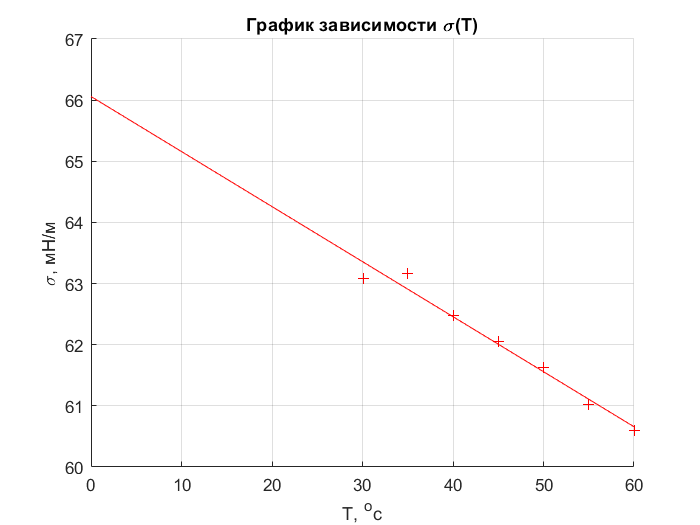
\includegraphics[scale=0.5]{plot_1.png}
\end{center}
 Константа b в данной задаче определяет температурный коэффициент $\dfrac{d \sigma}{dT}$, $\dfrac{d \sigma}{dT} = -0,09\dfrac{\text{мН}}{\text{м}\cdot ^0c }$ 
\item На другом графике построим зависимость от температуры
\begin{enumerate}
\item теплоты образования единицы поверхности жидкости $q = -T \cdot \dfrac{d \sigma}{dT}$
\item поверхностной энергии U единицы площади F: $\dfrac{U}{F} = \sigma - T \cdot\dfrac{d \sigma}{dT}$
\begin{center}
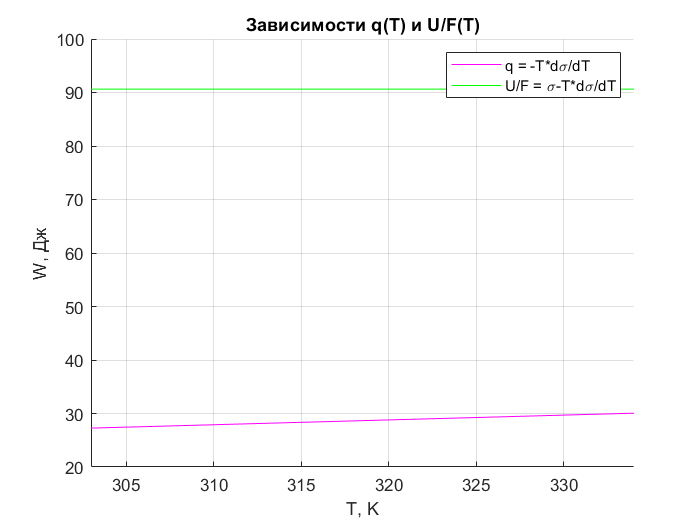
\includegraphics[scale=0.5]{plot_2.png}
\end{center}
\end{enumerate}
\end{enumerate}
\section{Вывод:}
\begin{enumerate}
\itemsep0em
\item Рассчитали диаметр иглы по формуле (\ref{laplass}) и по известному коэффициенту поверхностного натяжения спирта $$d = 1,05 \pm 0,02 \;\; \text{мм} $$
\item Установили линейную зависимость коэффициента поверхностного натяжения от температуры в данном диапазоне температур с погрешностью $\varepsilon = 2\%$
\item Рассчитали температурных коэффициент $$\dfrac{d\sigma}{dT} = -0,09 \frac{\text{мН}}{\text{м}\cdot K}$$ Табличное значение данного коэффициента равняется $$\dfrac{d\sigma_{T}}{dT} = -0,17 \frac{\text{мН}}{\text{м}\cdot K}$$ Расхождение в $\approx 50 \%$, вероятно, вызвано из-за того, что у нас не устанавливалось тепловое равновесие воды в термостате и воды, где происходил опыт. Также мы могли неточно рассчитать диаметр иглы или микроманометр был неисправен  
\end{enumerate}
\end{document}